%%%%%%%%%%%%%%%%%%%%%%%%%%%%%%%%%%%%%%%%%
% Beamer Presentation
% LaTeX Template
% Version 1.0 (10/11/12)
%
% This template has been downloaded from:
% http://www.LaTeXTemplates.com
%
% License:
% CC BY-NC-SA 3.0 (http://creativecommons.org/licenses/by-nc-sa/3.0/)
%
%%%%%%%%%%%%%%%%%%%%%%%%%%%%%%%%%%%%%%%%%

%----------------------------------------------------------------------------------------
%	PACKAGES AND THEMES
%----------------------------------------------------------------------------------------

\documentclass[UTF8,aspectratio=169,14pt]{ctexbeamer}

\usepackage{hyperref}
\hypersetup{
	colorlinks=true,
	linkcolor=red,
	anchorcolor=blue,
	citecolor=green
}

\mode<presentation> {
	
	% The Beamer class comes with a number of default slide themes
	% which change the colors and layouts of slides. Below this is a list
	% of all the themes, uncomment each in turn to see what they look like.
	
	%\usetheme{default}
	%\usetheme{AnnArbor}
	%\usetheme{Antibes}
	%\usetheme{Bergen}
	%\usetheme{Berkeley}
	%\usetheme{Berlin}
	%\usetheme{Boadilla}
	%\usetheme{CambridgeUS}
	%\usetheme{Copenhagen}
	%\usetheme{Darmstadt}
	%\usetheme{Dresden}
	%\usetheme{Frankfurt}
	%\usetheme{Goettingen}
	%\usetheme{Hannover}
	%\usetheme{Ilmenau}
	%\usetheme{JuanLesPins}
	%\usetheme{Luebeck}
	\usetheme{Madrid}
	%\usetheme{Malmoe}
	%\usetheme{Marburg}
	%\usetheme{Montpellier}
	%\usetheme{PaloAlto}
	%\usetheme{Pittsburgh}
	%\usetheme{Rochester}
	%\usetheme{Singapore}
	%\usetheme{Szeged}
	%\usetheme{Warsaw}
	
	% As well as themes, the Beamer class has a number of color themes
	% for any slide theme. Uncomment each of these in turn to see how it
	% changes the colors of your current slide theme.
	
	%\usecolortheme{albatross}
	%\usecolortheme{beaver}
	%\usecolortheme{beetle}
	%\usecolortheme{crane}
	%\usecolortheme{dolphin}
	%\usecolortheme{dove}
	%\usecolortheme{fly}
	%\usecolortheme{lily}
	%\usecolortheme{orchid}
	%\usecolortheme{rose}
	%\usecolortheme{seagull}
	%\usecolortheme{seahorse}
	%\usecolortheme{whale}
	%\usecolortheme{wolverine}
	
	%\setbeamertemplate{footline} % To remove the footer line in all slides uncomment this line
	%\setbeamertemplate{footline}[page number] % To replace the footer line in all slides with a simple slide count uncomment this line
	
	%\setbeamertemplate{navigation symbols}{} % To remove the navigation symbols from the bottom of all slides uncomment this line
}

\usepackage{graphicx} % Allows including images
\graphicspath{{./figs/}}
\usepackage{booktabs} % Allows the use of \toprule, \midrule and \bottomrule in tables
\usepackage{longtable}
\usepackage{listings}
\usepackage{xcolor}
\lstset{numbers=left, %设置行号位置
	numberstyle=\tiny, %设置行号大小
	keywordstyle=\color{blue}, %设置关键字颜色
	commentstyle=\color[cmyk]{1,0,1,0}, %设置注释颜色
	frame=single, %设置边框格式
	escapeinside=``, %逃逸字符(1左面的键),用于显示中文
	%breaklines, %自动折行
	extendedchars=false, %解决代码跨页时,章节标题,页眉等汉字不显示的问题
	xleftmargin=2em,xrightmargin=2em, aboveskip=1em, %设置边距
	tabsize=4, %设置tab空格数
	showspaces=false %不显示空格
}
% Fonts
% \usepackage{libertine}
% \setmonofont{Courier}
\setCJKsansfont[ItalicFont=Noto Serif CJK SC Black, BoldFont=Noto Sans CJK SC Black]{Noto Sans CJK SC}


%----------------------------------------------------------------------------------------
%	TITLE PAGE
%----------------------------------------------------------------------------------------

\title[第16讲]{第十六讲 :进程通信} % The short title appears at the bottom of every slide, the full title is only on the title page
\subtitle{第5节:D-Bus机制}
\author{向勇、陈渝、李国良} % Your name
\institute[清华大学] % Your institution as it will appear on the bottom of every slide, may be shorthand to save space
{
	清华大学计算机系 \\ % Your institution for the title page
	\medskip
	\textit{xyong,yuchen,liguoliang@tsinghua.edu.cn} % Your email address
}
\date{\today} % Date, can be changed to a custom date

\begin{document}

\begin{frame}
\titlepage % Print the title page as the first slide
\end{frame}

%----------------------------------------------
%\begin{frame}
%\frametitle{提纲} % Table of contents slide, comment this block out to remove it
%\tableofcontents % Throughout your presentation, if you choose to use \section{} and \subsection{} commands, these will automatically be printed on this slide as an overview of your presentation
%\end{frame}
%----------------------------------------------
%%	PRESENTATION SLIDES
%----------------------------------------------
\section{第4节:D-Bus机制} % Sections can be created in order to organize your presentation into discrete blocks, all sections and subsections are automatically printed in the table of contents as an overview of the talk
%----------------------------------------------
\subsection{D-Bus介绍} % A subsection can be created just before a set of slides with a common theme to further break down your presentation into chunks
%----------------------------------------------
\begin{frame}[fragile]
    \frametitle{D-Bus介绍}
%    \framesubtitle{xxxx}

	\begin{columns}
	\begin{column}{.4\textwidth}
		
	
\includegraphics[width=.6\textwidth]{redhat-fd}
	
\includegraphics[width=.3\textwidth]{gnome3}
	
\includegraphics[width=.3\textwidth]{kde}	
	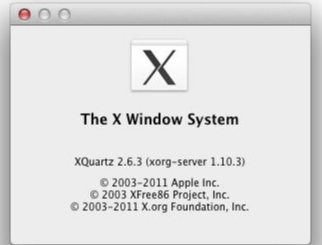
\includegraphics[width=.3\textwidth]{x11}
	\end{column}
	\begin{column}{.6\textwidth}
		\large
    \begin{itemize}
        \item 2002年创建的一种进程间通信机制
        \item 是freedesktop.org项目的一部分
        \item 有Redhat和FreeDesktop社区维护
		\item 主要Linux桌面环境中的通信服务
    \end{itemize}
	\end{column}
	\end{columns}
\end{frame}
%----------------------------------------------
\begin{frame}[fragile]
	\frametitle{D-Bus介绍}
	%    \framesubtitle{xxxx}
	
	\begin{columns}
		\begin{column}{.5\textwidth}
			\begin{itemize}
			\item 早期的IPC机制
			\item socket相对使用广泛
			\item 某些机制已经很少使用
			\end{itemize}			
			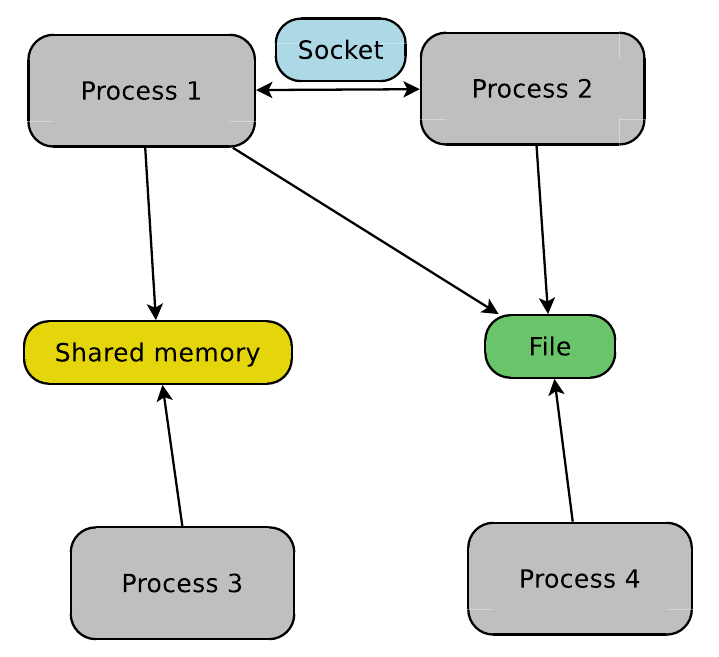
\includegraphics[width=.75\textwidth]{normal-ipc}
			
		\end{column}
		\pause
		\begin{column}{.5\textwidth}
			\begin{itemize}
				\item 使用socket机制
				\item 提供了软件总线抽象
				\item 比传统IPC机制简单
			\end{itemize}
			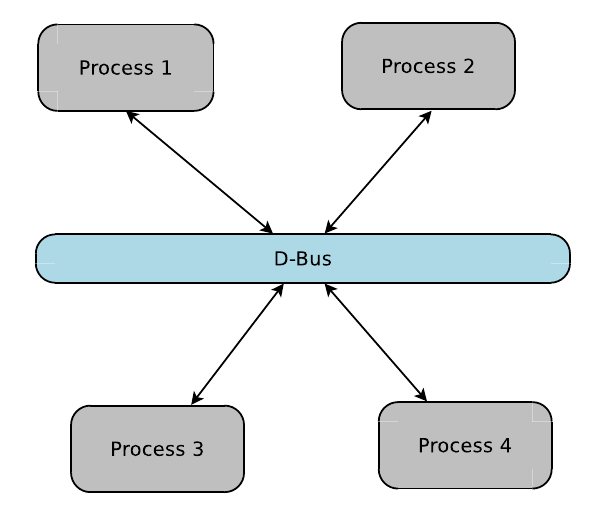
\includegraphics[width=.8\textwidth]{dbus-ipc}
		\end{column}
	\end{columns}
\end{frame}

%----------------------------------------------
\begin{frame}[fragile]
	\frametitle{D-Bus介绍}
	%    \framesubtitle{xxxx}
	
	\begin{columns}
		\begin{column}{.4\textwidth}
			
			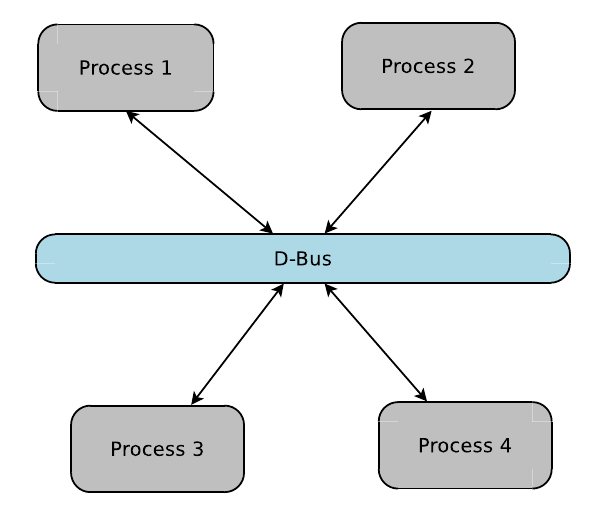
\includegraphics[width=1.\textwidth]{dbus-ipc}
			
		\end{column}
		\begin{column}{.6\textwidth}
%			\large
			基本特征
			\begin{itemize}
				\item 高层次的IPC
				\item Multicast \& point-to-point
				\item OS/architecture/language无关
				\item GNOME, KDE, xfce
			\end{itemize}
			优势
			\begin{itemize}
				\item 低延迟:无socket的循环的等待
				\item 低开销:使用一个二进制的协议
				\item 高可用性:基于消息机制而不是字节流机制
			\end{itemize}
		\end{column}
	\end{columns}
\end{frame}
%----------------------------------------------
%----------------------------------------------
\begin{frame}[fragile]
	\frametitle{D-Bus运行机制}
	%    \framesubtitle{xxxx}
	
	\begin{columns}
		\begin{column}{.4\textwidth}
			
			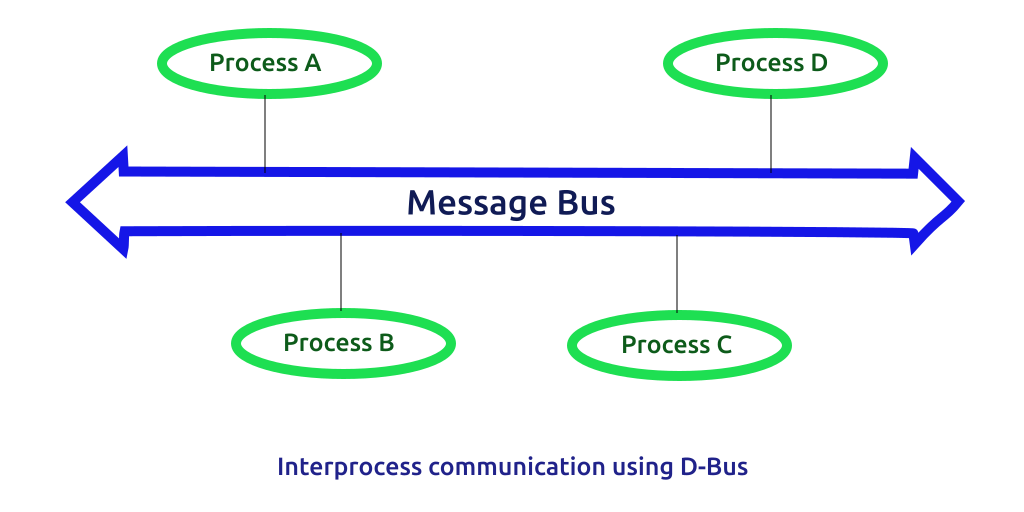
\includegraphics[width=.8\textwidth]{dbus-simple}
			\includegraphics[width=.8\textwidth]{dbus-diagram}
			
		\end{column}
		\begin{column}{.6\textwidth}
%			\large
			D-Bus结构
			\begin{itemize}
				\item 一个库libdbus,它允许两个应用程序相互连接并交换消息
				\item 一个消息总线守护程序(daemon),建立在libdbus,多个应用程序可以连接到
				\item 包装程序库或基于特定应用程序框架的绑定
				\item System Bus \& Session Bus
				\item 通过policy文件制定安全机制

			\end{itemize}
		\end{column}
	\end{columns}
\end{frame}

%----------------------------------------------
\begin{frame}[plain]
	\frametitle{D-Bus运行机制}
    \begin{figure}
    \centering
    \includegraphics[width=.63\textwidth]{dbus-diagram}
    %\caption{D-Bus的组成:总线、服务、对象、接口、方法和信号}
    \end{figure}
    \centering D-Bus的组成:总线、服务、对象、接口、方法和信号

\end{frame}
%----------------------------------------------
\begin{frame}[fragile]
	\frametitle{D-Bus运行机制}
	%    \framesubtitle{xxxx}
	
	\begin{columns}
		\begin{column}{.4\textwidth}
			
			\includegraphics[width=1.\textwidth]{dbus-diagram}
			
		\end{column}
		\begin{column}{.6\textwidth}
			%			\large
			D-Bus的总线(bus):D-BUS的通信链路,应用之间通过总线进行通信,应用在总线上寻找服务
            \begin{itemize}
                \item 系统总线(System Bus)
                \begin{itemize}
                    \item 用于kernel、系统应用/服务
                \end{itemize}
                \item 任务总线 (Session Bus)
                \begin{itemize}
                    \item 用于gnome/kde等应用通信
                \end{itemize}
            \end{itemize}
		\end{column}
	\end{columns}
\end{frame}

%----------------------------------------------
\begin{frame}[fragile]
	\frametitle{D-Bus运行机制}
	%    \framesubtitle{xxxx}
	
	\begin{columns}
		\begin{column}{.4\textwidth}
			
			\includegraphics[width=1.\textwidth]{dbus-diagram}
			
		\end{column}
		\begin{column}{.6\textwidth}
			%			\large
			D-Bus的服务(service)
			\begin{itemize}
				\item 提供IPC API的程序:每个服务都有一个reverse domain name结构的标识名称
				\item org.freedesktop.NetworkManager对应系统总线上的NetworkManager
				\item org.freedesktop.login1对应系统总线上的systemd-logind
				
			\end{itemize}
		\end{column}
	\end{columns}
\end{frame}

%----------------------------------------------
\begin{frame}[fragile]
	\frametitle{D-Bus运行机制}
	%    \framesubtitle{xxxx}
	
	\begin{columns}
		\begin{column}{.4\textwidth}
			
			\includegraphics[width=1.\textwidth]{dbus-diagram}
			
		\end{column}
		\begin{column}{.6\textwidth}
			%			\large
			D-Bus的对象(object)
			\begin{itemize}
				\item 通信地址:每个service的object都通过object path来标识
				\item object path类似文件系统的路径
				\item 如服务org.freedesktop.login1的manager对象路径为/org/freedesktop/login1
				
			\end{itemize}
		\end{column}
	\end{columns}
\end{frame}

%----------------------------------------------
\begin{frame}[fragile]
	\frametitle{D-Bus运行机制}
	%    \framesubtitle{xxxx}
	
	\begin{columns}
		\begin{column}{.4\textwidth}
			
			\includegraphics[width=1.\textwidth]{dbus-diagram}
			
		\end{column}
		\begin{column}{.6\textwidth}
			%			\large
			D-Bus的接口(interface)
			\begin{itemize}
				\item 定义D-Bus对象支持的方法(method)和信号(signal)
				\item 每个D-Bus对象包含一个或者多个接口				
			\end{itemize}
		\end{column}
	\end{columns}
\end{frame}

%----------------------------------------------
\begin{frame}[fragile]
	\frametitle{D-Bus运行机制}
	%    \framesubtitle{xxxx}
	
	\begin{columns}
		\begin{column}{.4\textwidth}
			
			\includegraphics[width=1.\textwidth]{dbus-diagram}
			
		\end{column}
		\begin{column}{.6\textwidth}
			%			\large
			D-Bus的方法(method)
			\begin{itemize}
				\item D-Bus方法可以接受任意数量的参数,并且可以返回任意数量的值,包括任何值。				
			\end{itemize}
			D-Bus的信号(signal)
			\begin{itemize}
				\item D-Bus信号提供了一对多的发布-订阅机制
				\item 与方法返回值类似,D-Bus信号可能包含任意数量的数据
				\item 与方法不同,信号是完全异步的,并且可以随时由D-Bus对象发出 			
			\end{itemize}		
		\end{column}
	\end{columns}
\end{frame}

%----------------------------------------------
\begin{frame}[fragile]
	\frametitle{D-Bus运行机制}
	%    \framesubtitle{xxxx}
	
	\begin{columns}
		\begin{column}{.4\textwidth}
			
			\includegraphics[width=1.\textwidth]{dbus-diagram}
			
		\end{column}
		\begin{column}{.6\textwidth}
			%			\large
			D-Bus方法的执行流程
			\begin{itemize}				
				\item 应用调用代理上的方法,代理将构造一个方法调用消息给远端的进程
				\item 方法调用消息发送到bus daemon中
				\item bus daemon查找目标的bus name,如果找到,就把这个方法发送到该进程中
				\item D-Bus高层接口会先检测并转换成对应的对象的方法,然后再将应答结果转换成应答消息发给daemon
				\item bus daemon接受到应答消息,将把应答消息直接发给发出调用消息的进程		
			\end{itemize}		
		\end{column}
	\end{columns}
\end{frame}
%----------------------------------------------
%----------------------------------------------
\end{document}
